\chapter*{Preface}
\addcontentsline{toc}{chapter}{Preface} % Add the preface to the table of contents as a chapter


The finite element method (FEM) is by now one of the most popular
methods for numerically solving Partial Differential Equations (PDEs) in
science, engineering and applied mathematics. There are a number of
good reasons for this:

\begin{itemize}
	\item[\Smiley] For \textbf{elliptic}
	and \textbf{parabolic} problems\sidenote[][-0.2cm]{\textbf{Elliptic problems}:
		Stationary diffusion,
		heat conduction, fully developed laminar flows in ducts,
		linear elasticity.\\
		\textbf{Parabolic problems}:
		Transient diffusion or heat conduction, chemical kinetics,
		fluid dynamics.},
	the FEM provides very accurate solutions;\\
	
	\item[\Smiley] It is \textbf{general}, not restricted to linear problems,
	or to isotropic problems, or to any subclass of mathematical
	problems; \\
	
	\item[\Smiley] It is \textbf{geometrically flexible}, complex domains
	are quite easily treated, not requiring adaptations of the
	method itself; \\
	
	\item[\Smiley] It is \textbf{easy to code}, and the coding is quite problem-independent.
	Boundary conditions are much easier to deal with than in other methods; \\
	
	\item[\Smiley] It is \textbf{robust}, because in most cases the mathematical problem
	has an underlying variational structure (energy minimization, for example). \\
	
\end{itemize}

\begin{marginfigure}[-4.0cm]
	\hrule
	\vspace{0.1cm}
	\flushleft \textbf{\scriptsize Solid mechanics}
	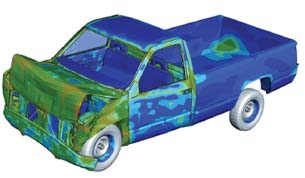
\includegraphics[width=0.8\textwidth]{truck}
	\vspace{0.1cm}       
	\hrule
	\vspace{0.1cm}
	\textbf{\scriptsize Heat transfer}
	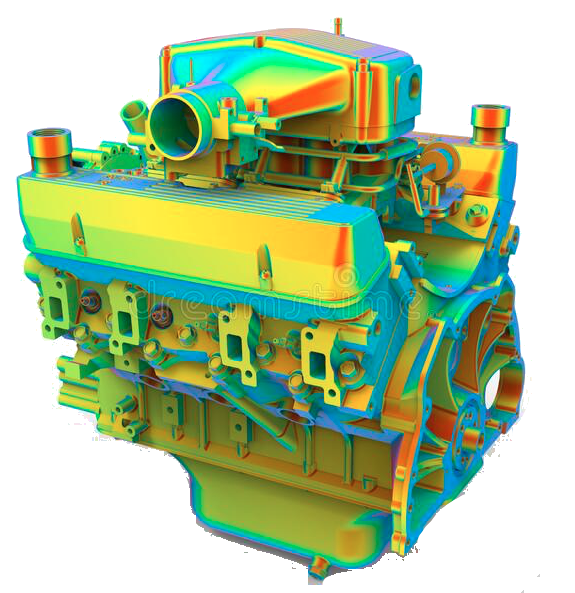
\includegraphics[width=0.7\textwidth]{engine2}
	\vspace{0.1cm}       
	\hrule
	\vspace{0.1cm}
	\textbf{\scriptsize Internal flows: Turbomachinery}
	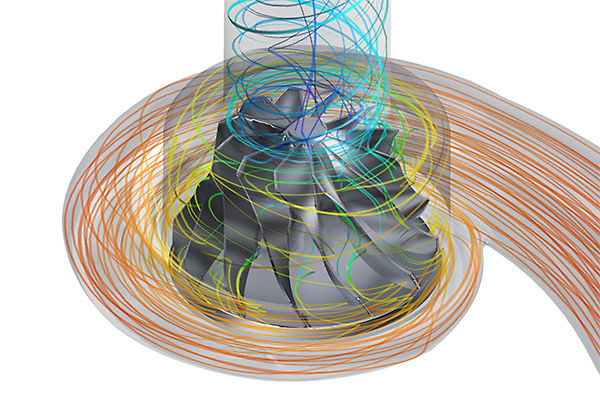
\includegraphics[width=0.8\textwidth]{turbine3}
	\vspace{0.1cm}
	\hrule
	\vspace{0.1cm}
	\textbf{\scriptsize Computational hemodynamics}
	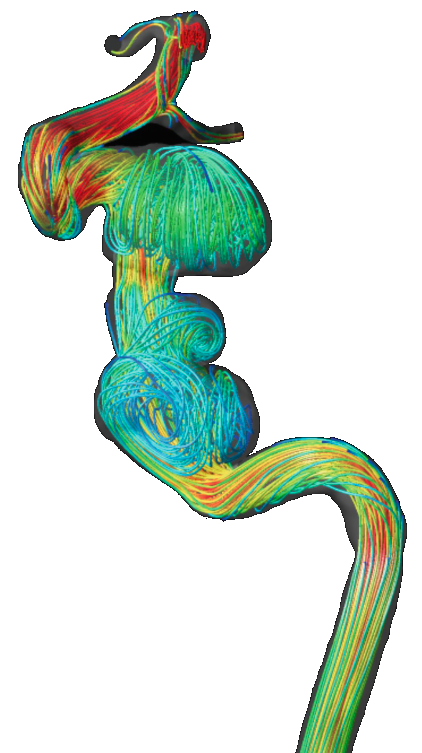
\includegraphics[width=0.5\textwidth,angle=90]{hemodyn2}
	\vspace{0.1cm}~\\
	\hrule
	\vspace{0.1cm}
	\textbf{\scriptsize External flows: Aerodynamics}
	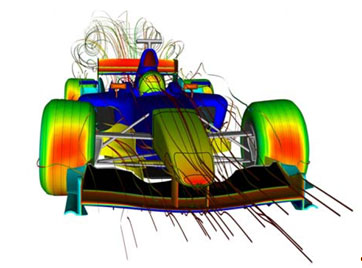
\includegraphics[width=0.8\textwidth]{f1formula}
	\vspace{0.1cm} 
	\hrule
	\caption[]{Examples solved by FEM.}
	\labfig{examples}
\end{marginfigure}

\section{What This Course Covers}
\labsec{does}

The main objective of this course is to introduce the student to the \href{https://fenicsproject.org/}{\texttt{FEniCSx}} open source platform for solving PDEs using the Finite Element method, through practical examples that arise in Solid and Fluid Mechanics.
The \texttt{FEniCS} project is a high-end open source platform that allows you to efficiently automate the resolution of partial differential equations (PDEs) by the finite element method (FEM). By using  a domain-specific language called UFL (Uniform Form Language) it is possible to write the variational formulation of complex problems governed by PDEs and their discretization by the FEM. Despite using a high-level language, the library allows solving problems efficiently with parallel computing, since it generates code in C that is compiled at runtime to perform the assembly of matrices and vectors that emerges when the FEM is applied. 

This course consists of a series of practical lectures to demonstrate the use 
of the software and its potential to solve some relevant 2nd order PDEs 
of interest in fluid and solid mechanics.  
Although the main focus of the course is practical (it will be a hands-on course), some mathematical and theoretical aspects will be recalled so as to provide the necessary context to understand the physical/mathematical problems considered and their numerical resolution by the finite element method. The target audience for the course is primarily graduate students, however, advanced undergrads in applied mathematics, physics or engineering courses are welcome to take the course. Students are expected to have minimal knowledge about PDEs and the physical models behind the problems to be solved. Some previous background about discretization methods for PDEs is also desirable.

The course will be divided into 5 lectures with the following topics to be covered: 

\begin{description}
	\item[Lecture |01|] Introduction:
	\begin{itemize}
		\item Examples of PDEs in fluid and solid mechanics
		\item Preliminary notions on the Finite Element Method
		\item The \texttt{FEniCSx} platform
		\item A first example: The heat conduction equation
	\end{itemize}
	
	\item[Lecture |02|] Classical problems:
	\begin{itemize}
		\item Transient heat conduction equation
		\item The elasticity problem
	\end{itemize}
	
	\item[Lecture |03|] Mixed problems:
	\begin{itemize}
		\item Coupled thermo-elasticity problem
		\item The Navier-Stokes equations
	\end{itemize}
	
	\item[Lecture |04|] Advanced topics:	
	\begin{itemize}
		\item Darcy's flow: $H(\mbox{div})$ formulations;
		\item Electromagnetism: The Helmholtz equation: 
	\end{itemize}
	
	\item[Lecture |05|] High Performance Computing with \texttt{FEniCSx}:	
	\begin{itemize}
		\item Notions on parallel computing
		\item Scalability: Weak and Strong scaling
	\end{itemize}
	
\end{description}

Each lecture will be accompanied by a \texttt{Colab Notebook} 
available at the public repository 
\href{https://fenicsproject.org/}{\texttt{USP-FEniCSx-Course}},
in which some of the relevant mathematical concepts that are part of 
this document will be recalled. At the end of each lecture, there is a
\textbf{Homework assignment} that must be presented the day after
to the corresponding lecture. 

\begin{kaobox}[frametitle=Disclaimer]	
	The following notes are not intended to be a comprehensive
	exposition of the theory and practice of the finite element method,
	but only a summary of some relevant concepts of interest for this
	course. For a complete description, the student is referred to 
	\cite{ern-guermond,ciarlet,Reddy,Brenner}.
\end{kaobox}

\begin{flushright}
	\textit{RFA \& IAB} 
\end{flushright}
